\documentclass[12pt]{article}

% fonts
\usepackage{graphicx, subfigure, caption}
\usepackage[scaled=0.92]{helvet}   % set Helvetica as the sans-serif font
\usepackage{tikz}
\usepackage[colorlinks=true,
            linkcolor=red,
            urlcolor=blue]{hyperref}
\usetikzlibrary{shapes,arrows}
\renewcommand{\rmdefault}{ptm}     % set Times as the default text font

% graphical models
% \usepackage{tikz}
% \usetikzlibrary{bayesnet}

% dmb: not mandatory, but i recommend you use mtpro for math fonts.
% there is a free version called mtprolite.

% \usepackage[amssymbols,subscriptcorrection,slantedGreek,nofontinfo]{mtpro2}


\usepackage[T1]{fontenc}
\usepackage{amsmath}
\usepackage{amsfonts}

% page numbers
\usepackage{fancyhdr}
\fancypagestyle{newstyle}{
\fancyhf{} % clear all header and footer fields
\fancyfoot[R]{\vspace{0.1in} \small \thepage}
\renewcommand{\headrulewidth}{0pt}
\renewcommand{\footrulewidth}{0pt}}
\pagestyle{newstyle}

% geometry of the page
\usepackage[top=1in, bottom=1in, left=1.625in, right=1.625in]{geometry}

% paragraph spacing
\setlength{\parindent}{0pt}
\setlength{\parskip}{2ex plus 0.4ex minus 0.2ex}

% lists
\providecommand{\tightlist}{%
  \setlength{\itemsep}{0pt}\setlength{\parskip}{0pt}}

% useful packages
\usepackage{natbib}
\usepackage{epsfig}
\usepackage{url}
\usepackage{bm}
\begin{document}

\begin{center}
  \Large \textbf{Probabilistic Detection of Character Voices in Fiction} \\
  \vspace{0.1in}
  \normalsize J. Reeve \\
  \today
\end{center}

In James Joyce's novel \emph{Ulysses}, the school headmaster Mr.~Deasy
quotes Shakespeare in a lecture in financial responsibility to his
employee Stephen Dedalus. ``{[}W{]}hat does Shakespeare say?'' he asks,
``Put but money in thy purse.'' As Stephen remembers it, however, this
is not merely a saying of Shakespeare's, but one spoken by Shakespeare's
infamous character Iago. So while Deasy thinks himself to be quoting the
wisdom of the early modern playwright, he is, in fact, quoting the
Bard's most notorious arch-villain. This distinction---one between an
author and the author's fictional creations---is, it need not be said,
crucial to the understanding of literature. It is that which the
following experiment hopes to probabilistically detect.

The problem of computational character attribution is one of literary
knowledge production. In concrete terms, it is the difference between
the sentence ``Madam, I never eat muscatel grapes'' and its TEI XML
markup,
\texttt{\textless{}said\ who="Edmond\ Dantès"\textgreater{}Madam,\ I\ never\ eat\ muscatel\ grapes\textless{}/said\textgreater{}}.
In the first case, a reader familiar with \emph{The Count of Monte
Cristo} might recognize it as spoken by Edmond Dantès, in the second
case, the reader need not know the work to attribute the sentence to its
speaker. This markup allows for answers to a wide range of questions,
such as the size of the work's cast of characters, the distribution of
character speech, and stylistic properties of an individual character.
These are queries that are useful for both close and distant
reading---they can provide insight about particular characters and a
novel as a whole. They are useful both to the close study of a single
work and to the distant study of hundreds or thousands of novels at a
time. This markup, although a laborious task for a human annotator,
might be generated semi-automatically from stylistic signatures of the
character.

\section{Experimental Design}\label{experimental-design}

The design of this series of experiments is based on Box's Loop, an
iterative process for refining a probabilistic model based on its
predictive performance {[}@blei\_build\_2014 205{]}. The meta-analysis
is one of model selection, analysis, model criticism, and improvement,
while the analysis itself consists of four steps: chunking, vectorizing,
dimensionality reduction, and prediction. Chunking involves the choice
of documents, and the modification of those documents to fit certain
lengths. Each document only contains text in one character's voice, but
these documents might be of varying length. Vectorizing is the
transformation of those documents into numeric representations, whether
through traditional ``bag-of-words'' term frequency representations or
more semantic techniques. Dimensionality reduction transforms those
high-dimensional vectors into lower-dimensional ones that are more
easily manipulable by the predictive step. Prediction takes the
transformed set of vectors and performs probabilistic inference,
effectively assigning character voices to each document.

For each of these steps, there are many available techniques and
parameters. To identify the best ones, I used a cross-validation grid
search that performs a meta-analysis by testing all permutations of
these techniques. \footnote{A full list of techniques and parameters
  tested may be found in the project repository, in
  \href{https://github.com/JonathanReeve/character-attribution/blob/master/waves/waves-grid-search-meta.ipynb}{the
  grid search notebooks for The Waves} and
  \href{https://github.com/JonathanReeve/character-attribution/blob/master/clarissa/clarissa-grid-search.ipynb}{for
  Clarissa}} The grid search tests each configuration against an
adjusted Rand score comparison of the labeled data with its predicted
clusters. This metric accounts for chance, so that a score close to zero
indicates a parameter configuration that performs no better than chance,
while a score close to 1 is a perfect clustering, identical with the
clustering of the original labels, although not necessarily labeled
identically.

To test the efficacy of voice detection, we use two TEI XML texts,
distant from each other in time and genre: Virginia Woolf's experimental
1931 novel, \emph{The Waves} and Samuel Richardson's classic 1748
epistolary novel \emph{Clarissa}. \emph{The Waves} is notable in that it
is almost all monologue spoken by six characters. \emph{Clarissa} is
composed almost entirely of letters, mostly from four of the novel's
approximately 30 characters. These novels were chosen simply because
they were already available in TEI XML format, which made possible the
extraction of substantial amounts of labeled text in their characters'
voices.

\section{The Waves}\label{the-waves}

A manual, preliminary parameter search showed that character attribution
worked best with utterances longer than four thousand characters.
Furthermore, very long utterances, such as Bernard's 66,000-character
speech that ends the novel, threw off the analysis. With this in mind, I
restricted the total 240 utterances of \emph{The Waves} to just the 19
that were between 2000 and 20000 characters in length. The lengths of
these documents conform roughly to a normal distribution, with a mean of
6487 characters, and a standard deviation of 1960.

From there, I vectorized these documents using a TF-IDF vectorizer,
which counts the frequency of each word, and reweights these according
to how frequently they are used in the corpus. I set a maximum document
frequency of 30\% to ignore corpus-specific stop words, and then limit
the vocabulary to the top 500 words (these are parameters suggested by
the cross-validation search). The resulting vectors I then reduce to
five dimensions using principal component analysis. This 19x5 matrix
become the input for probabilistic inference. A two-dimensional
projection of this matrix is shown in Figure 1 (a), with each point
representing a single character's utterance. Of note here is the
apparent separation in this projection between the male and female
characters, with the male characters in the upper right and the female
characters in the lower left.

\begin{figure}
\centering   
\subfigure[Initial Labels]{\label{fig:a}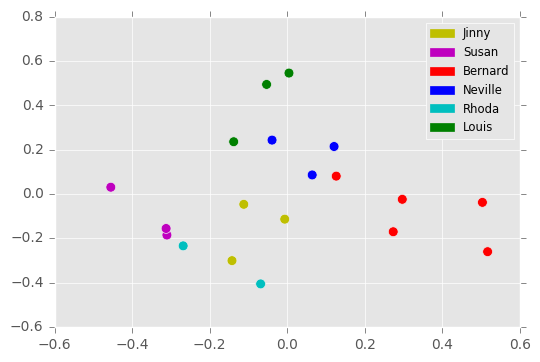
\includegraphics[width=120mm]{../charts/waves-e2-labeled}}
\subfigure[Final Convergence]{\label{fig:c}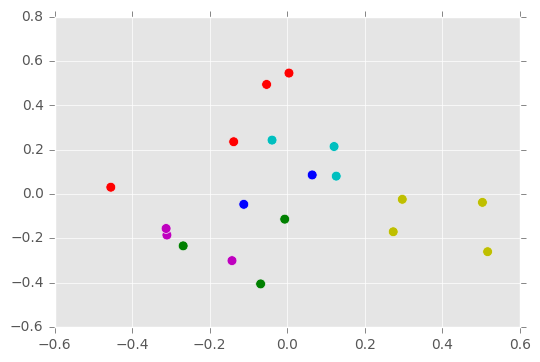
\includegraphics[width=120mm]{../charts/waves-e2-final}}
\caption{Character Clusterings in The Waves}
\end{figure}

The probabilistic model used for clustering assumes that the
dimension-reduced, TF-IDF-weighted word frequencies can be modeled with
a mixture of Gaussians. I performed inference using scikit-learn's
\texttt{GaussianMixture} class, which uses the expectation-maximization
(EM) algorithm to cluster the data. Given six components in which to
cluster data, the class clustered the data into the six groups shown in
Figure 1 (b). The labels aren't identical with the original labels in
Figure 1 (b), but the groupings are similar. The inference correctly
groups together four out of five of Bernard's utterances, three out of
four of Louis's, two out of three of Neville's, Rhoda's, and Susan's,
but misidentifies Jinny's. After twenty trials with this configuration,
the mean adjusted Rand score was 0.443, with a standard deviation of
0.076---performing better than chance, although not perfectly\footnote{The
  code used for this analysis, written in the Python programming
  language and using the Scikit-Learn machine learning library, is
  available at
  \href{https://github.com/JonathanReeve/character-attribution/blob/master/clarissa/clarissa-grid-search.ipynb}{this
  project's GitHub repository}}.

\section{Clarissa}\label{clarissa}

After manually tagging and extracting character-labeled letters from
Richardson's \emph{Clarissa}, I generated test documents by selecting
only letters longer than 8,000 characters and shorter than 50,000
characters. This produced a corpus of 180 letters of varying lengths,
the respective lengths of which are indicated by the sizes of the dots
in Figure 2. I then vectorized these documents using the top 500 most
frequently used words, and reduced the resulting matrix to 25 principal
components using PCA, the first two dimensions of which are shown in
Figure 2 (a). As in the \emph{Waves} experiment, these were all
parameters suggested by the cross-validation grid search. Unlike the
Waves experiment, however, the grid search suggested a slightly
different inference model: a Bayesian Gaussian mixture model. This model
differs from the \texttt{GaussianMixtureModel} class in that it uses
variational inference. Additionally, it doesn't always provide the
number of clusters requested, but only no more than those requested.

Curiously, the grid search suggested that we request that the Bayesian
Gaussian mixture model provide four clusters, fewer than the number of
characters. However, this turned out to have not been an error, since
the amount of text represented by the relatively minor characters James
and Morden (as evidenced by the paucity of green and red dots in Figure
2 (a) is very small, and it would almost be fair to assume that there
are really only four characters represented here.

The final clustering is shown in Figure 2 (b). It incorrectly clusters
together the correspondence of villains Lovelace and Belford, but
forgivably, since these characters are friends and associates, and at
most points in the novel partners in crime. It correctly identifies most
of Anna's correspondence, but divides her best friend Clarissa's into
two groups: one closer to Anna, and another closer to Lovelace. A closer
analysis, which is perhaps beyond the scope of the present experiment,
might reveal that those of Clarissa's letters closest to Anna's are
letters in fact written to Anna, while her letters that appear closest
to Belford and Lovelace might, in fact, be those written to them. In
fact, the clustering here, though inaccurate, might be more useful to
literary analysis than an accurate clustering: they might reveal not
only the character voices themselves, but degrees or modes of these
voices. They might show how voice changes according to addressee.

\begin{figure}
\centering   
\subfigure[Initial Labels]{\label{fig:a}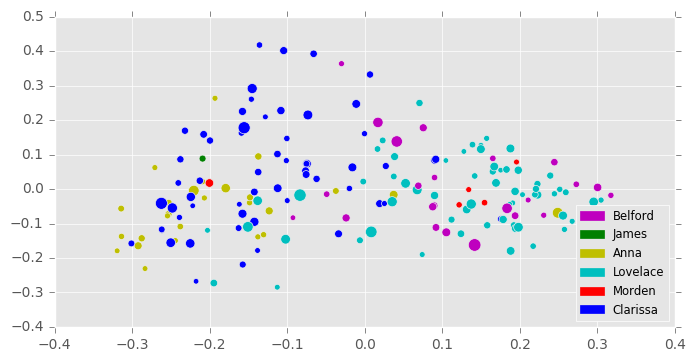
\includegraphics[width=120mm]{../charts/clarissa-e2-labeled}}
\subfigure[Final Convergence]{\label{fig:b}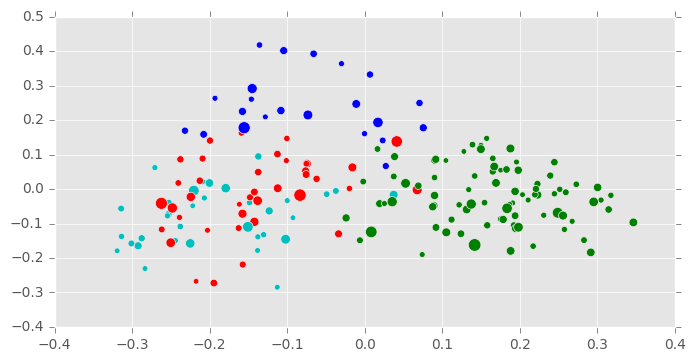
\includegraphics[width=120mm]{../charts/clarissa-e2-final}}
\caption{Character Clusterings in Clarissa}
\end{figure}

The adjusted Rand score for this clustering is a slightly lower 0.357,
faring much better than chance, but still worse than \emph{The Waves}.
Although these experiments used different parameters and clustering
techniques, this discrepancy might be telling.

\section{Beyond Bag-of-Words}\label{beyond-bag-of-words}

The experiments above all rely on word frequency representations of
text, and often only on the frequencies of the top 500 words (most
likely function words). But what if other properties of the words, such
as their meanings, were taken into account? First, I tried transforming
documents into 300-dimensional vector representations using the GloVe
algorithm in the SpaCy natural language processing Python
library\footnote{See {[}@pennington\_glove:\_2014{]} for more on GloVe,
  and {[}@turian\_word\_2010{]} for more on word vector embeddings in
  general.}. The best configuration for this representation, an
experiment run on the top four characters, reducing the dimensions to 5
with PCA, and performing inference with a Gaussian mixture model with
four components, showed a mean adjusted Rand score of 0.192, with a
standard deviation of 0.023 after twenty trials. Figure 3 (b) shows the
results of that experiment. Here, the probabilistic inference manages to
separate, at the 0.0 longitudinal line, protagonists from antagonists,
and male from female characters, grouping Anna and Clarissa together,
and Lovelace and Belford. It does not seem to be able to distinguish
between those individual characters, however.

\begin{figure}
\centering   
\subfigure[Initial Labels]{\label{fig:a}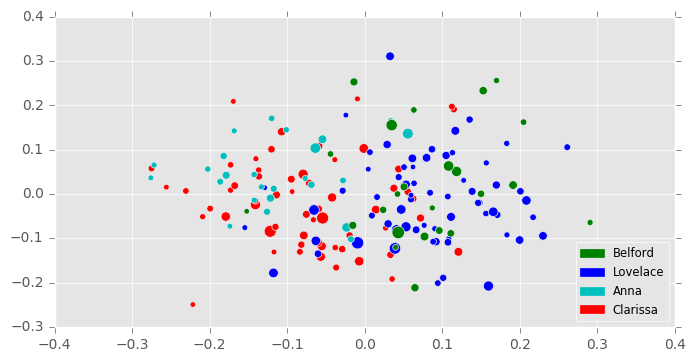
\includegraphics[width=120mm]{../charts/clarissa-vec1-labeled}}
\subfigure[Final Convergence]{\label{fig:b}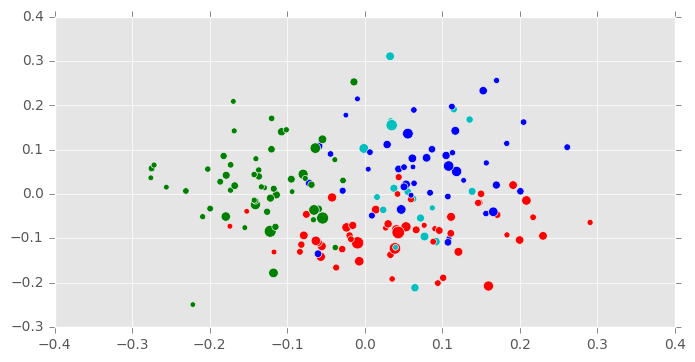
\includegraphics[width=120mm]{../charts/clarissa-vec1-final}}
\caption{Character Clusterings with Semantic Word Vector Transformations}
\end{figure}

I attempted other vectorizations, as well, without much success. A
representation of a document as a vector of parts of speech frequencies
produced scores roughly equal to those of chance. Another vectorization
that represented documents as the frequencies of the root words in each
sentence performed equally poorly. Since semantic word vectorizations
performed only about half as well as the word frequency vectorizations
described above, and similar representations even worse, we must
conclude that character voice is most discernible in the frequencies of
function words, rather than in the meanings of the words.

\section{Discussion}\label{discussion}

The difference in the highest possible adjusted rand scores for each
novel---0.443 for \emph{The Waves}, and 0.357 for \emph{Clarissa}, might
be a useful observation. Perhaps the respective scores indicate the
degree to which a writer is able to write in the styles of his or her
characters. Conversely, this difference might indicate the degree to
which a writer's choice of characters is stylistically different. If
that is the case, novelists with many classes of broadly-painted
characters such as Charles Dickens might show higher scores than
novelists like Jane Austen who deal with the social subtleties.

Although the technique outlined this paper might not be appropriate for
fully unsupervised character voice attribution, some manual tagging of
groups might help to automate speaker attribution somewhat. In any case,
attributions of very small utterances (with fewer than 2,000 characters)
may not be possible with this word frequency representation.

If these techniques do not prove to be very useful in automating
character voice attributions, however, they might be useful to literary
studies in another way. By examining the confusion caused by certain
probabilistic clusterings, we might be able to infer groups of
characters---male and female characters, for instance, or protagonists
and antagonists. By using an unsupervised model such as the Bayesian
Gaussian model used with \emph{Clarissa}, we might also be able to
infer, with some small degree of confidence, the numbers of main
characters.

\end{document}
